
\providecommand{\QCat}{\mathcal{Q}\mathit{Cat}}%
\providecommand{\hQCat}{\mathfrak{h}\QCat}%
\providecommand{\Hom}{\operatorname{Hom}}%

\section{伴随}\label{sec:f-adjunctions}

拟范畴间伴随的解析定义与综合定义之间的比较，比本附录中所考察的其他范畴论
概念要微妙一些，因为这两者通常是以不同的数据来陈述的。伴随的综合定义原本
归于 Joyal \cite{bib63}，它涉及两个指定的函子 $f\colon B\to A$ 与
$u\colon A\to B$，连同指定的映射 $\eta\colon B\times\Delta[1]\to B$ 与
$\epsilon\colon A\times\Delta[1]\to A$\footnote{原书两处均印作「$\eta$」；
按\cref{prop:synthetic-analytic-adjunction}(i) 中 $\eta\colon\mathrm{id}_{B}\Rightarrow uf$
与 $\epsilon\colon fu\Rightarrow\mathrm{id}_{A}$ 之记号分工，第二处疑为
$\epsilon$ 之误，此处径改。——译者注}——在 $B^{B}$ 或 $A^{A}$ 中至差一个
同伦——再连同拟范畴 $B^{A}$ 与 $A^{B}$ 中见证\trTriangleEqualities{}的
2-\trSimplex{}。与此相对，$A$ 与 $B$ 之间伴随的解析概念归于 Lurie
\cite[5.2.2.1]{bib78}，它被定义为一条等价纤维化\footnote{爱挑剔的读者或许
会注意到，Lurie 只要求一个\trInnerFibration，但 $\Delta[1]$ 之上的任何\trInnerFibration{}都
自动是等价纤维化。事实上，只要 $M$ 是一个拟范畴，任何单纯映射
$M\to\Delta[1]$ 都自动是等价纤维化。} $M\twoheadrightarrow\Delta[1]$，它
同时是一条\trCartesianFibration{}与一条\trCocartesianFibration，称为一个
\textbf{\trCorrespondence}（correspondence），并配有等价 $M_{1}\simeq A$ 与
$M_{0}\simeq B$，把拟范畴 $A$ 与 $B$ 等同于该 1-\trSimplex{}两端点之上的
诸\trFiber。

由于\cref{prop:adjunction-equivalence-invariant}证明了伴随的综合概念是等价
不变的，我们稍微简化一下记号，令 $B$ 与 $A$ 表示等价纤维化
$M\twoheadrightarrow\Delta[1]$ 在 0 与 1 之上的诸\trFiber。本节的目标是
证明：从一条余笛卡尔与笛卡尔纤维化 $M\twoheadrightarrow\Delta[1]$ 出发，
可以提取出一个 $B$ 与 $A$ 之间的\trAdjunction，其伴随函子在\trIsomorphism{}%
的意义下被唯一确定；反之，从一个 2-范畴式的\trAdjunction{}出发，可以构造出
一个相应的\trCorrespondence{} $M\twoheadrightarrow\Delta[1]$，其在\trFiberedEquivalence{}%
的意义下唯一。由于证明更为繁难，我们把论证拆成若干个中间步骤。

\begin{proposition}\label{prop:correspondence-adjunction}
设 $M$ 是一个配有映射 $M\twoheadrightarrow\Delta[1]$ 的\trQuasiCategory，
该映射同时是一条\trCocartesianFibration{}与\trCartesianFibration。那么
\begin{itemize}
\item 诸\trFiber{} $B\coloneqq M_{0}$ 与 $A\coloneqq M_{1}$，以及
\item 由 $\Delta[1]$ 中泛箭头的余笛卡尔\trLifting{}与笛卡尔\trLifting{}%
分别定义的诸\trFunctor{} $f\colon B\to A$ 与 $u\colon A\to B$
\end{itemize}
定义一个\trAdjunction
\begin{center}
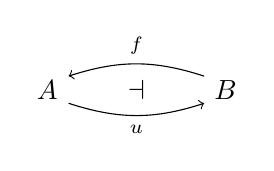
\begin{tikzpicture}[x=1.4em,y=1.4em]
  \node (A) at (0,0)   {$A$};
  \node (B) at (4.6,0) {$B$};
  \draw[->] (4.05,0.35) to[bend right=18] node[above]{$\scriptstyle f$} (0.55,0.35);
  \node at (2.3,0) {$\dashv$};
  \draw[->] (0.55,-0.35) to[bend right=18] node[below]{$\scriptstyle u$} (4.05,-0.35);
\end{tikzpicture}
\end{center}
\end{proposition}

\begin{proof}
这是\cref{prop:bifibration-fibered-adjunction}的一个特例。我们回顾 $f$ 与
$u$ 的构造，而把其余细节留给该结果与\cref{rem:fiber-action}。设 $\chi$
表示 $\Delta[1]$ 中泛箭头的一支余笛卡尔\trLifting，其定义域是 0 之上的%
\trFiber{}之包含 $B\hookrightarrow M$。这条被提升箭头的陪域落入 1 之上
的\trFiber{}之中，从而经该\trFiber{}的包含 $A\hookrightarrow M$ 唯一地分解：
\begin{center}
\begin{tikzpicture}[x=1.9em,y=1.5em]
  \node (B)  at (0,1.4)    {$B$};
  \node (M)  at (3.2,1.4)  {$M$};
  \node (One) at (0,-1.4)  {$1$};
  \node (D1) at (3.2,-1.4) {$\Delta[1]$};
  \draw[->] (0.45,1.85) to[bend left=20] (2.75,1.85);
  \node at (0.55,0.8) {$\scriptstyle\llcorner$};
  \draw[->] (0,1.0) -- (0,-1.0);
  \draw[->] (3.2,1.0) -- (3.2,-1.0);
  \draw[->] (0.6,-1.05) to[bend left=22] node[above]{$\scriptstyle 0$} (2.6,-1.05);
  \node at (1.6,-1.5) {$\scriptstyle\Downarrow\psi$};
  \draw[->] (0.6,-1.8) -- node[below]{$\scriptstyle 1$} (2.6,-1.8);
  \node at (5.1,0) {$=$};
  \begin{scope}[shift={(7.0,0)}]
  \node (B2) at (0,1.4)    {$B$};
  \node (M2) at (3.2,1.4)  {$M$};
  \node (Ax) at (1.6,0.1)  {$A$};
  \node (O2) at (0,-1.4)   {$1$};
  \node (D2) at (3.2,-1.4) {$\Delta[1]$};
  \draw[->,dashed] (0.45,1.85) to[bend left=20] node[above]{$\scriptstyle\psi\chi$} (2.75,1.85);
  \draw[->] (0.35,0.95) -- node[left,pos=0.55]{$\scriptstyle f$} (1.25,0.42);
  \draw[right hook->] (1.95,0.42) -- (2.9,1.0);
  \node at (2.5,0.55) {$\scriptstyle\llcorner$};
  \draw[->] (0,1.0) -- (0,-1.0);
  \draw[->] (3.2,1.0) -- (3.2,-1.0);
  \draw[->] (0.6,-1.05) to[bend left=22] node[below]{$\scriptstyle 1$} (2.6,-1.05);
  \end{scope}
\end{tikzpicture}
\end{center}
这一分解定义了\trFunctor{} $f\colon B\to A$。由于一支固定箭头的诸余笛卡尔%
\trLifting{}与一个固定\trFunctor{}的诸\trAdjunction{}各自都在%
\trIsomorphism{}的意义下唯一，这一构造是适当良定义的。\trRightAdjoint{}
$u\colon A\to B$ 的构造是对偶的，涉及 $\Delta[1]$ 中泛箭头的一支笛卡尔%
\trLifting。
\end{proof}

逆命题用到了我们称为\textbf{拟范畴\trCollage{}构造}（quasi-categorical collage
construction）的东西。

\begin{definition}[拟范畴\trCollage{}构造]\label{def:quasicategorical-collage}
对拟范畴之间的任意余跨度 $B\xrightarrow{g}C\xleftarrow{f}A$\footnote{原书两杆
均印作指向左，与定义条件及 p.728 证明之 $g\colon B\to C$ 不合，此处径改。
——译者注}，定义一个单纯集
$\mathrm{col}(f,g)$ 如下：
\[
\mathrm{col}(f,g)_{n}=\Bigl\{(a\in A_{i},\,b\in B_{j},\,c\in C_{n})\;\Bigm|\;
\begin{array}{l}
c_{[0,\dotsc,i]}=f(a),\ i,j\ge -1,\\
c_{[n-j,\dotsc,n]}=g(b),\ i+j=n-1
\end{array}\Bigr\}
\]
其中约定由 $\Delta[-1]$ 编号的条件为空（或者说每个单纯集都是末端增广的）。
有显然的包含纳入如下交换图：
\begin{center}
\begin{tikzpicture}[x=1.9em,y=1.5em]
  \node (B)  at (0,1.4)    {$B$};
  \node (C)  at (3.4,1.4)  {$\mathrm{col}(f,g)$};
  \node (A)  at (6.8,1.4)  {$A$};
  \node (B1) at (0,-1.4)   {$\{1\}$};
  \node (D)  at (3.4,-1.4) {$\Delta[1]$};
  \node (Z)  at (6.8,-1.4) {$\{0\}$};
  \draw[right hook->] (0.5,1.4) -- (2.2,1.4);
  \draw[right hook->] (6.3,1.4) -- (4.6,1.4);
  \node at (0.65,0.75) {$\scriptstyle\llcorner$};
  \node at (6.15,0.75) {$\scriptstyle\llcorner$};
  \draw[->] (0,1.0) -- (0,-1.0);
  \draw[->] (3.4,1.0) -- (3.4,-1.0);
  \node at (3.85,0) {$\scriptstyle\rho$};
  \draw[->] (6.8,1.0) -- (6.8,-1.0);
  \draw[right hook->] (0.5,-1.4) -- (2.2,-1.4);
  \draw[right hook->] (6.3,-1.4) -- (4.6,-1.4);
\end{tikzpicture}
\end{center}
映射 $\rho$ 把 $n$ 单形 $(a\colon\Delta[i]\to A,\ b\colon\Delta[j]\to B,\ c\colon\Delta[n]\to C)$
送到把 $0,\dotsc,i$ 送到 0 而把 $i+1,\dotsc,n$ 送到 1 的那个 $n$ 单形
$[n]\to[1]$。注意，$\rho$ 在 0 之上的\trFiber{}\trIsomorphism{}于 $A$，而
$\rho$ 在 1 之上的\trFiber{}\trIsomorphism{}于 $B$。
\end{definition}

按照我们对\trTwoSidedFibration{}与\trModule{}的惯例，我们记 $B+A\hookrightarrow\mathrm{col}(f,g)$
为 1 与 0 之上的诸\trFiber{}之包含——1 之上的\trFiber{}在左，0 之上的%
\trFiber{}在右。这就把协变地作用的拟范畴置于「左」，而把反变地作用的拟范畴
置于「右」。

\begin{lemma}\label{lem:collage-inner-fibration}
映射 $\rho\colon\mathrm{col}(f,g)\to\Delta[1]$ 是一个\trInnerFibration。特别地，单纯集
$\mathrm{col}(f,g)$ 是一个\trQuasiCategory。
\end{lemma}

\begin{proof}
由于 $\rho$ 在 0 与 1 之上的诸\trFiber{}是拟范畴 $A$ 与 $B$，只需考虑内号角
\begin{center}
\begin{tikzpicture}[x=1.9em,y=1.5em]
  \node (L)  at (0,1.3)    {$\Lambda^{k}[n]$};
  \node (Cl) at (4.4,1.3)  {$\mathrm{col}(f,g)$};
  \node (Dn) at (0,-1.4)   {$\Delta[n]$};
  \node (D1) at (4.4,-1.4) {$\Delta[1]$};
  \draw[->] (1.2,1.3) -- (3.0,1.3);
  \draw[right hook->] (0,0.95) -- (0,-1.0);
  \draw[->] (1.2,-1.4) -- node[below]{$\scriptstyle\alpha$} (3.3,-1.4);
  \draw[->] (4.4,0.95) -- (4.4,-1.0);
  \node at (4.85,0) {$\scriptstyle\rho$};
  \draw[->,dashed] (0.5,-1.15) -- (3.9,1.05);
\end{tikzpicture}
\end{center}
其中 $\alpha\colon[n]\to[1]$ 是满射。设 $\alpha$ 把 $0,\dotsc,i$ 送到 0，把
$i+1,\dotsc,n$ 送到 1。注意，对任何 $0<k<n$，$\Delta[n]$ 的诸面
$\{0,\dotsc,i\}$ 与 $\{i+1,\dotsc,n\}$ 都属于号角 $\Lambda^{k}[n]$。特别地，
映射 $\Lambda^{k}[n]\to\mathrm{col}(f,g)$ 把单纯形 $a\colon\Delta[i]\to A$
与 $b\colon\Delta[n-i-1]\to B$ 连同一个号角 $\Lambda^{k}[n]\to C$ 一道等同
起来，该号角的初始面与最终面是这些单纯形在 $f\colon A\to C$ 与
$g\colon B\to C$ 之下的像。由于 $C$ 是拟范畴，这个号角容有一个填充体
$c\colon\Delta[n]\to C$，而三元组 $(a,b,c)$ 定义出 $\mathrm{col}(f,g)$ 中
解决该\trLifting{}问题的一个 $n$ 单形。
\end{proof}

我们记 $\mathrm{col}(f,B)$ 为 $f\colon A\to B$ 与 $B$ 上的恒同所成的\trCollage。

\begin{lemma}\label{lem:collage-cocartesian-fibration}
对任何 $f\colon A\to B$，映射 $\rho\colon\mathrm{col}(f,B)\to\Delta[1]$ 是
一条\trCocartesianFibration。
\end{lemma}

\begin{proof}
由\cref{prop:cartesian-fibration-analytic}(vi)，为证明本断言，我们只需指定
$\Delta[1]$ 的非退化 1-\trSimplex{}的诸余笛卡尔\trLifting，并证明这些边具有
相应的\trUniversalProperty。为此，对任何顶点 $a\in A_{0}$，设
$\chi_{a}\colon\Delta[1]\to\mathrm{col}(f,B)$ 是 1-\trSimplex
\[
\chi_{a}\coloneqq(a\colon\Delta[0]\to A,\ fa\colon\Delta[0]\to B,\ fa\sigma^{0}\colon\Delta[1]\to B),
\]
它由位于 $\Delta[1]$ 中该 1-\trSimplex{}之上的、$fa\in B_{0}$ 处的退化边
给出。为证 $\chi_{a}$ 是 $\rho$-\trCocartesian，我们必须为任何以 $\chi_{a}$
为初始边的左号角构造填充体
\begin{center}
\begin{tikzpicture}[x=1.9em,y=1.5em]
  \node (D1) at (0,1.3)    {$\Delta[1]$};
  \node (L)  at (3.6,1.3)  {$\Lambda^{0}[n]$};
  \node (Cl) at (7.6,1.3)  {$\mathrm{col}(f,B)$};
  \node (Dn) at (3.6,-1.4) {$\Delta[n]$};
  \node (D2) at (7.6,-1.4) {$\Delta[1]$};
  \draw[->] (1.1,1.3) -- node[below]{$\scriptstyle\{0,1\}$} (2.5,1.3);
  \draw[->] (4.7,1.3) -- (6.5,1.3);
  \draw[->] (0.5,1.8) to[bend left=18] node[above,pos=0.5]{$\scriptstyle\chi_{a}$} (7.1,1.8);
  \draw[right hook->] (3.6,0.95) -- (3.6,-1.0);
  \draw[->] (4.7,-1.4) -- node[below]{$\scriptstyle\beta$} (6.5,-1.4);
  \draw[->] (7.6,0.95) -- (7.6,-1.0);
  \node at (8.05,0) {$\scriptstyle\rho$};
  \draw[->,dashed] (4.0,-1.15) -- (7.1,1.05);
\end{tikzpicture}
\end{center}
注意，这一条件蕴含底映射 $\beta\colon[n]\to[1]$ 把 0 送到 0，而把其余顶点
送到 1。映射 $\Lambda^{0}[n]\to\mathrm{col}(f,B)$ 在拟范畴 $B$ 中定义了一个
号角 $\Lambda^{0}[n]\to B$，其首条边是退化的。由
\cref{prop:special-outer-horn-filling}，这个「特殊外号角」容有一个填充体
$b\colon\Delta[n]\to B$，而三元组
\[
(a\colon\Delta[0]\to A,\ b\sigma^{0}\colon\Delta[n-1]\to B,\ b\colon\Delta[n]\to B)
\]
定义出解决该\trLifting{}问题的 $\mathrm{col}(f,B)$ 中的一个 $n$ 单形。
\end{proof}

\begin{proposition}\label{prop:collage-oplax-colimit}
对拟范畴之间的任何 $f\colon A\to B$，\trCollage{} $\mathrm{col}(f,B)$ 定义 $f$ 在
$\QCat$ 中的\textbf{\trOplaxColimit}（oplax colimit）。也就是说，
$\mathrm{col}(f,B)$ 在如下推出图之下定义一个锥\footnote{图中虚线杆之标目
原书印作 $i_{1}\hat{p}$，与本页正文「诱导映射 $k$」不合（本节并无 F.4 节之
$E^{2}\twoheadrightarrow\mathrm{Hom}_{B}(B,p)$ 语境），疑为 F.4 节同名记号
之排印残留，此处照录原书面貌。——译者注}
\begin{center}
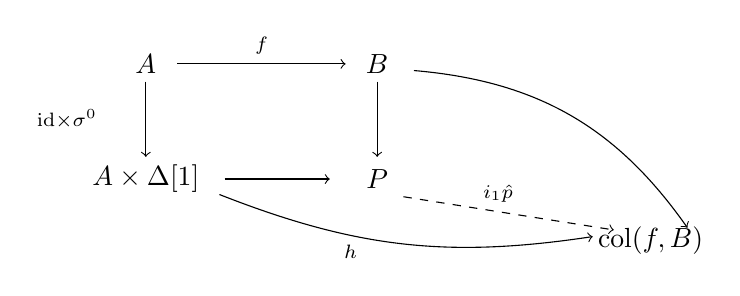
\begin{tikzpicture}[x=1.9em,y=1.6em]
  \node (A)  at (0,1.4)    {$A$};
  \node (B)  at (4.4,1.4)  {$B$};
  \node (AD) at (0,-1.2)   {$A\times\Delta[1]$};
  \node (P)  at (4.4,-1.2) {$P$};
  \node (Cl) at (9.6,-2.6) {$\mathrm{col}(f,B)$};
  \draw[->] (0.6,1.4) -- node[above]{$\scriptstyle f$} (3.8,1.4);
  \draw[->] (0,1.0) -- (0,-0.7);
  \node at (-1.5,0.15) {$\scriptstyle\mathrm{id}\times\sigma^{0}$};
  \draw[->] (4.4,1.0) -- (4.4,-0.7);
  \node at (2.9,0.35) {$\scriptstyle\llcorner$};
  \draw[->] (1.5,-1.2) -- (3.5,-1.2);
  \draw[->] (1.4,-1.55) to[bend right=15] node[below,pos=0.35]{$\scriptstyle h$} (8.5,-2.5);
  \draw[->] (5.1,1.25) to[bend left=25] (10.3,-2.3);
  \draw[->,dashed] (4.9,-1.6) -- node[above,pos=0.45]{$\scriptstyle i_{1}\hat{p}$} (8.9,-2.35);
\end{tikzpicture}
\end{center}
使得诱导映射 $k$ 是\trInnerAnodyne{}的，从而特别是在 Joyal \trModelStructure{}中
的一个\trWeakEquivalence。
\end{proposition}

\begin{proof}
映射 $k$ 是映射 $h$ 的一个商，后者有如下显式描述。对每个 $n$ 单形
$(a,\alpha)\colon\Delta[n]\to A\times\Delta[1]$，定义
$i\coloneqq\lvert\alpha^{-1}(0)\rvert-1$，从而 $-1\le i\le n$。那么 $h$ 把
$(a,\alpha)$ 送到 $\mathrm{col}(f,B)$ 的由如下三元组所对应的 $n$ 单形
\[
(a|_{[0,\dotsc,i]}\colon\Delta[i]\to A,\ fa|_{[i+1,\dotsc,n]}\colon\Delta[n-i-1]\to B,\ fa\colon\Delta[n]\to B).
\]
注意，复合 $\rho h\colon A\times\Delta[1]\to\Delta[1]$ 是投影。

剩下要做的是把 $k$ 呈现为内号角包含之余积的推出的一个序列复合。为此，首先
注意
\[
\mathrm{col}(f,B)_{n}=A_{n}\sqcup A_{n-1}\times_{B_{n-1}}B_{n}\sqcup\dotsb\sqcup A_{0}\times_{B_{0}}B_{n}\sqcup B_{n}
\]
其中每个映射 $B_{n}\to B_{i}$ 是对应于 $\{0,\dotsc,i\}\hookrightarrow\Delta[i]$
的初始面映射。在这一分解的视角下，$P_{n}$ 是这样一个子集：它含有诸集合
$A_{n}$ 与 $B_{n}$，以及 $A_{i}\times_{B_{i}}B_{n}$ 中其在 $B_{n}$ 中的分量
落在 $f$ 的像内的那个子集。$\mathrm{col}(f,B)$ 中尚待贴附的诸 $n$ 单形对应
于 $A_{i}\times_{B_{i}}B_{n}$（$0\le i<n$）中不属于刚才所论意义上的 $f$ 之
像的那些元素。特别值得注意的是，顶点上的映射
$k\colon P_{0}\hookrightarrow\mathrm{col}(f,B)_{0}$ 是一个\trIsomorphism，
而对一切 $n\ge 1$，$k\colon P_{n}\hookrightarrow\mathrm{col}(f,B)_{n}$ 是
一个单射。

为枚举我们的贴附映射，我们从 $\mathrm{col}(f,B)$ 中非退化的诸 $n$ 单形
（$n\ge 1$）不在 $f$ 的像内者的集合出发，并再剔除 $A_{i}\times_{B_{i}}B_{n}$
中其分量 $b\in B_{n}$ 落在退化映射 $\sigma_{i}\colon B_{n-1}\to B_{n}$ 的像
内的那些元素。将这一单纯形集合先按 $n$ 递增的顺序、继而按标号 $i$ 递增的
顺序偏序化；也就是说，我们对二元组 $(n,i)$（$n\ge 1$，$0\le i<n$）之集合
按字典序排序。

我们把包含 $P\hookrightarrow\mathrm{col}(f,B)$ 滤过为
\[
\begin{gathered}
P\hookrightarrow P_{(1,0)}\hookrightarrow P_{(2,0)}\hookrightarrow P_{(2,1)}\hookrightarrow P_{(3,0)}\hookrightarrow\dotsb\\
\dotsb\hookrightarrow P_{(n,i)}\hookrightarrow\dotsb\hookrightarrow\mathrm{colim}\simeq\mathrm{col}(f,B)
\end{gathered}
\]
其中单纯集 $P_{(n,i)}$ 由前一个经一个推出构造而得，该推出所用的内号角之
余积以 $b$ 不在 $f$ 或 $\sigma_{i}$ 的像内的诸 $n$ 单形
$(a,b)\in A_{i}\times_{B_{i}}B_{n}$ 之集合为指标。以 $(a,b)$ 为标目的号角之
填充体将把这个 $n$ 单形作为号角的缺失面贴附到 $B_{n}$ 上，并且同时贴附
$n+1$ 单形 $(a,b\sigma^{i})\in A_{i}\times_{B_{i}}B_{n+1}$。

考虑一个 $b$ 不在 $f$ 或 $\sigma_{i}$ 的像内的单纯形
$(a,b)\in A_{i}\times_{B_{i}}B_{n}$。定义一个号角
\begin{center}
\begin{tikzpicture}[x=1.9em,y=1.5em]
  \node (L)  at (0,1.3)    {$\Lambda^{i+1}[n+1]$};
  \node (P)  at (5.8,1.3)  {$P_{(n,i)}$};
  \node (D)  at (0,-1.5)   {$\Delta[n+1]$};
  \node (Cl) at (5.8,-1.5) {$\mathrm{col}(f,B)$};
  \draw[->] (2.6,1.3) -- (4.4,1.3);
  \draw[right hook->] (0,0.95) -- (0,-1.1);
  \draw[right hook->] (5.8,0.95) -- (5.8,-1.1);
  \draw[->] (1.7,-1.5) -- node[below]{$\scriptstyle(a,b\sigma^{i})$} (4.4,-1.5);
\end{tikzpicture}
\end{center}
对每个 $0\le j<i+1$，$n+1$ 单形 $(a,b\sigma^{i})$ 的 $\delta^{j}$ 面是
$n$ 单形 $(a\delta^{j},\,b\sigma^{i}\delta^{j})$，它落于 $P_{(n,i-1)}$ 之中，
或在 $i=0$ 的情形落于 $B\hookrightarrow P$ 之中。对每个 $i+1<j\le n+1$，
$n+1$ 单形 $(a,b\sigma^{i})$ 的 $\delta^{j}$ 面是 $n$ 单形
$(a,\,b\sigma^{i}\delta^{j})=(a,\,b\delta^{j-1}\sigma^{i})\in A_{i}\times_{B_{i}}B_{n}$，
它此前已被贴附到 $P_{(n-1,i)}$。于是，号角 $\Lambda^{i+1}[n+1]$ 确实映入
$P_{(n,i)}$，这使得本序列中的下一个单纯集可以归纳地构造为如下推出
\begin{center}
\begin{tikzpicture}[x=1.9em,y=1.5em]
  \node (L)  at (0,1.3)    {$\amalg\Lambda^{i+1}[n+1]$};
  \node (P)  at (6.6,1.3)  {$P_{(n,i)}$};
  \node (D)  at (0,-1.6)   {$\amalg\Delta[n+1]$};
  \node (P1) at (6.6,-1.6) {$P_{(n,i)+1}$};
  \draw[->] (3.6,1.3) -- (5.3,1.3);
  \draw[right hook->] (0,0.95) -- (0,-1.2);
  \draw[->] (6.6,0.95) -- (6.6,-1.2);
  \draw[->] (2.9,-1.6) -- (5.2,-1.6);
  \node at (5.5,-0.35) {$\scriptstyle\llcorner$};
\end{tikzpicture}
\end{center}
其中 $P_{(n,i)+1}$ 在 $i=n-1$ 的情形是 $P_{(n+1,0)}$，否则是 $P_{(n,i+1)}$。
\end{proof}

把这些结果拢在一起，我们如今便能证明伴随的综合概念与解析概念之间所求的
等价性。

\begin{proposition}\label{prop:synthetic-analytic-adjunction}
对拟范畴之间的一对\trFunctor{} $f\colon B\to A$ 与 $u\colon A\to B$，以下
诸条件等价，并且定义了拥有如下一个\trAdjunction{}的含义
\begin{center}
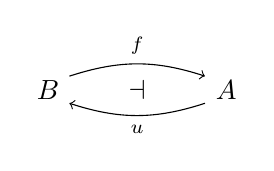
\begin{tikzpicture}[x=1.4em,y=1.4em]
  \node (B) at (0,0)   {$B$};
  \node (A) at (4.6,0) {$A$};
  \draw[->] (0.55,0.35) to[bend left=18] node[above]{$\scriptstyle f$} (4.05,0.35);
  \node at (2.3,0) {$\dashv$};
  \draw[->] (4.05,-0.35) to[bend left=18] node[below]{$\scriptstyle u$} (0.55,-0.35);
\end{tikzpicture}
\end{center}
\begin{enumerate}[label=(\roman*)]
\item 存在\trNaturalTransformation{} $\eta\colon\mathrm{id}_{B}\Rightarrow uf$
与 $\epsilon\colon fu\Rightarrow\mathrm{id}_{A}$，满足\trTriangleEqualities{}：
$u\epsilon\cdot\eta u=\mathrm{id}_{u}$ 与 $\epsilon f\cdot f\eta=\mathrm{id}_{f}$。
\item \trFunctor{} $f$ 定义 $\mathrm{id}_{B}$ 经 $u$ 的一个\trAbsoluteLeftLifting：
\begin{center}
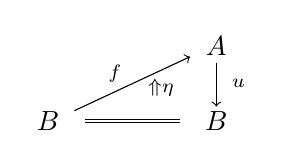
\begin{tikzpicture}[x=1.9em,y=1.5em]
  \node (A)  at (3.2,1.4)  {$A$};
  \node (B)  at (0,-0.4)   {$B$};
  \node (B2) at (3.2,-0.4) {$B$};
  \draw[->] (0.5,-0.15) -- node[above,pos=0.35]{$\scriptstyle f$} (2.7,1.15);
  \draw[->] (3.2,1.0) -- (3.2,-0.05);
  \node at (3.62,0.5) {$\scriptstyle u$};
  \node at (2.15,0.4) {$\scriptstyle\Uparrow\eta$};
  \draw[double] (0.7,-0.4) -- (2.5,-0.4);
\end{tikzpicture}
\end{center}
\item \trFunctor{} $u$ 定义 $\mathrm{id}_{A}$ 经 $f$ 的一个\trAbsoluteRightLifting：
\begin{center}
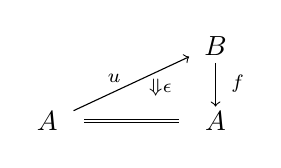
\begin{tikzpicture}[x=1.9em,y=1.5em]
  \node (B)  at (3.2,1.4)  {$B$};
  \node (A)  at (0,-0.4)   {$A$};
  \node (A2) at (3.2,-0.4) {$A$};
  \draw[->] (0.5,-0.15) -- node[above,pos=0.35]{$\scriptstyle u$} (2.7,1.15);
  \draw[->] (3.2,1.0) -- (3.2,-0.05);
  \node at (3.62,0.5) {$\scriptstyle f$};
  \node at (2.15,0.4) {$\scriptstyle\Downarrow\epsilon$};
  \draw[double] (0.7,-0.4) -- (2.5,-0.4);
\end{tikzpicture}
\end{center}
\item 存在一个绝对的逐点左扩张图表：
\begin{center}
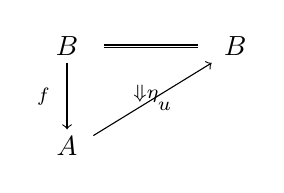
\begin{tikzpicture}[x=1.9em,y=1.5em]
  \node (B)  at (0,1.4)   {$B$};
  \node (B2) at (3.2,1.4) {$B$};
  \node (A)  at (0,-1.0)  {$A$};
  \draw[double] (0.7,1.4) -- (2.5,1.4);
  \draw[->] (0,1.0) -- (0,-0.6);
  \node at (-0.45,0.2) {$\scriptstyle f$};
  \draw[->] (0.5,-0.75) -- node[below,pos=0.6]{$\scriptstyle u$} (2.75,1.0);
  \node at (1.5,0.25) {$\scriptstyle\Downarrow\eta$};
\end{tikzpicture}
\end{center}
\item 存在一个绝对的逐点右扩张图表：
\begin{center}
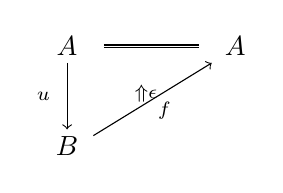
\begin{tikzpicture}[x=1.9em,y=1.5em]
  \node (A)  at (0,1.4)   {$A$};
  \node (A2) at (3.2,1.4) {$A$};
  \node (B)  at (0,-1.0)  {$B$};
  \draw[double] (0.7,1.4) -- (2.5,1.4);
  \draw[->] (0,1.0) -- (0,-0.6);
  \node at (-0.45,0.2) {$\scriptstyle u$};
  \draw[->] (0.5,-0.75) -- node[below,pos=0.6]{$\scriptstyle f$} (2.75,1.0);
  \node at (1.5,0.25) {$\scriptstyle\Uparrow\epsilon$};
\end{tikzpicture}
\end{center}
\item 诸\trModule{} $\Hom_{A}(f,A)\cong_{A\times B}\Hom_{B}(B,u)$ 在
$A\times B$ 之上等价。
\item \trCollage{} $\mathrm{col}(f,A)$ 与 $\mathrm{col}(B,u)$ 在 $A+B$ 之下且在
$\Delta[1]$ 之上等价，此时 $\mathrm{col}(f,A)\twoheadrightarrow\Delta[1]$
或等价地 $\mathrm{col}(B,u)\twoheadrightarrow\Delta[1]$ 同时定义一条%
\trCocartesianFibration{}与一条\trCartesianFibration。
\end{enumerate}
\end{proposition}

\begin{proof}
(i) 与 (ii) 或 (iii) 之间的等价性证明于\cref{lem:unit-counit-absolute-liftings}，
而与 (iv) 或 (v) 的等价性则证明于
\cref{prop:adjunction-counit-characterizations}。(i) 与 (vi) 之间的等价性
证明于\cref{prop:adjunction-as-fibered-equivalence}。我们最后证明 (i) 等价
于 (vii)。

首先设 $\mathrm{col}(f,A)\simeq\mathrm{col}(B,u)$ 在 $A+B$ 之下且在
$\Delta[1]$ 之上。由\cref{lem:collage-cocartesian-fibration}与
\cref{cor:equivalence-invariance}，这意味着映射 $\mathrm{col}(f,A)\to\Delta[1]$
同时是一条\trCocartesianFibration{}与一条\trCartesianFibration。由
\cref{prop:correspondence-adjunction}，$\Delta[1]$ 中从 0 到 1 的 1-箭头便
在诸\trFiber{} $B$ 与 $A$ 之间诱导出一个\trAdjunction。对该证明稍作检视
即知：就\trBifibration{} $\mathrm{col}(f,A)\to\Delta[1]$ 而论，如此构造出的%
\trLeftAdjoint{}函子正是 $f$；代入等价的\trBifibration
$\mathrm{col}(B,u)\to\Delta[1]$，便知\trRightAdjoint{}等价于 $u$。于是
(vii) 蕴含 (i)。

对于逆命题，我们在相反的\trInfinityCosmos{} $\QCat^{\mathrm{op}}$——一个
「并非所有对象都\trCofibrant」的\trInfinityCosmos，如 \cite{bib110} 所
描述——中进行工作。在这一语境下，\cref{prop:collage-oplax-colimit}证明了
$\mathrm{col}(f,A)$ 与 $\mathrm{col}(B,u)$ 构造的是与函子 $f$ 和 $u$
相关联的反变与协变逗号对象。若 $f\dashv u$（于 $\QCat$ 中），则这些函子在
$\QCat^{\mathrm{op}}$ 中也构成伴随，从而
\cref{prop:adjunction-as-fibered-equivalence}便证明诸逗号
$\mathrm{col}(f,A)$ 与 $\mathrm{col}(B,u)$ 在 $A+B$ 之下等价。由构造，这一
等价亦位于 $\Delta[1]$ 之上。或者，若读者不愿取对偶，也可以证明
$\mathrm{col}(f,A)$ 与 $\mathrm{col}(B,u)$ 定义了\trHomotopyTwoCategory{}
$\hQCat$ 中的「弱余逗号对象」，满足\cref{prop:comma-weak-universal-property}
之弱\trUniversalProperty{}的 1-范畴对偶。借助这些弱\trUniversalProperty，
\cref{prop:adjunction-as-fibered-equivalence}的证明可以在对偶中重复进行，
以构造出在 $A+B$ 之下且在 $\Delta[1]$ 之上所求的等价
$\mathrm{col}(f,A)\simeq\mathrm{col}(B,u)$。于是 (i) 蕴含 (vii)，证明完毕。
\end{proof}

\subsection*{练习}

\begin{exercise}\label{ex:correspondence-terminal-element}
构造一个\trCorrespondence，使之编码表达\trTerminal{}\trElement{}之\trUniversalProperty{}%
的那个\trAdjunction。
\end{exercise}

